\section{Introduction}

In Chapter \ref{sec:DTrepresentations_Volterra}, several competing representations were discussed for Volterra series modeling in the frequency domain, where each representation offers different benefits for interpretation and estimation \citep{Rijlaarsdam2017}, \citep{Cheng2017}. The GFRFs give perhaps the most natural representation, being multidimensional Fourier transforms of their corresponding time domain Volterra kernels ~\citep{George1959}. However, due to the complex multidimensional nature of the GFRFs, the NOFRF model was proposed \cite{Lang2005} to increase the ease of system analysis.  The model (see (\ref{eq:NOFRF_TransientFree})) contains only one-dimensional frequency functions which have a more intuitive interpretation from the perspective of linear systems theory, however, the functions are input dependent in general. This input dependence has restricted the use of NOFRFs to cases where input behaviour remains uniform over time, such as fault detection applications \citep{Peng2007}, \citep{Cao2013}, \citep{Xia2015} and nonlinearity detection \citep{Lang2008}. 

The NOFRF model proposal  in \cite{Lang2005} was accompanied by a data-driven identification algorithm, which uses multi-level excitation to estimate NOFRFs in a regression framework. This traditional method requires multiple experiments on the system under conditions that may not be possible in practice if the system excitation cannot be precisely controlled. The method also employs a least squares estimator that is sensitive to noisy measurements. In the special case of parallel Hammerstein systems it is possible to perform more sophisticated estimation, since the NOFRFs become independent of the applied input and the form of the functions closely resemble that of the underlying linear filters in the system's block structure. This property allows us to adopt well-developed concepts from linear identification theory.

The Bayesian regularization method for FIR estimation \cite{Pillonetto2010}, which provided the framework for contributions in Part \ref{part:TD} of this thesis, also has a linear frequency domain interpretation. Developed in \cite{Lataire2016}, the frequency domain method considers estimation of FRFs via Gaussian process regression (GPR). However, some additional challenges arise in the frequency domain case, due to the emergence of a transient function in the output spectrum when using non-steady-state data and the mixture of real and complex parameters contained in the FRF parameter vector. The results in \cite{Lataire2016} will provide a foundation for many of the contributions contained in Part \ref{part:FD} of the thesis. 

In this chapter, a GPR method is developed for estimating NOFRFs in the special case of a parallel Hammerstein system. The method is an extension to the linear frequency domain method in \cite{Lataire2016}. By framing the NOFRFs as normally distributed quantities with standard prior covariance structures, we can estimate all NOFRFs in a regularized fashion using only one experiment and with less restrictions than the traditional multi-level excitation method. Numerical examples reveal that the method proposed here is also significantly less sensitive to measurement noise than the traditional method in \cite{Lang2005}. The general case of non-steady-state data is also considered, where the GPR approach can be adapted to minimize the effect of transients on NOFRF estimation. 

The proposed method is distinct from other parallel Hammerstein identification algorithms in that it is a fully nonparametric method applied directly in the frequency domain. Traditionally, the linear dynamic and nonlinear blocks are estimated separately, and parametrically, in an iterative scheme \cite{Gallman1975}, \cite{Schoukens2011}, however the resulting models do not provide direct intuition on frequency domain behaviour. More recently, GPR has been applied to Hammerstein identification in the time domain~\cite{Risuleo2017}, but the approach was limited to a single Hammerstein branch.

\section{Real/complex normal distributions}
\label{sec:RCN}

The parameter vectors considered in the current chapter, as well as Chapter \ref{chap:8}, are free to contain both real and complex parameters. In order to express the distribution of Gaussian random vectors that contain both real and complex entries, the complex normal distribution \cite{Schreier2010} is not sufficient, since the associated augmented covariance matrix will be singular. Consequently, a hybrid Real/Complex Gaussian (RCG) distribution framework was developed in \cite{Lataire2016}, which will also be used in the sequel for parameter estimation. In this section we define some relevant notation and properties to enhance the readability of Chapters \ref{chap:7} and \ref{chap:8}. 

\begin{defn}[Real/Complex Gaussian vector]
A random vector
\begin{equation}
\label{eqn:RCG_vector_defn}
X = \begin{bmatrix} {X^{\mathbb{R}}} \\ {X^{\mathbb{C}}} \end{bmatrix}, \; \; \; X^{\mathbb{R}} \in \mathbb{R}^{n_r}, \; X^{\mathbb{C}} \in \mathbb{C}^{n_c}
\end{equation}
is said to be a RCG vector if the vector $$\begin{bmatrix} {X^{\mathbb{R}}} \\ \mathfrak{R}{X^{\mathbb{C}}} \\ \mathfrak{I}{X^{\mathbb{C}}} \end{bmatrix}$$ is Gaussian distributed, where $\mathfrak{R}$ and $\mathfrak{I}$ give the real and imaginary parts respectively. 
\end{defn}

\begin{notation}[Augmented vector]
For a RCG vector, $X$, the augmented vector is defined as 
\begin{equation}
\widetilde{X} = \begin{bmatrix} {X^{\mathbb{R}}} \\ {X^{\mathbb{C}}} \\ \bar{X}^{\mathbb{C}} \end{bmatrix}, 
\label{eq:augvector_defn}
\end{equation}
where $\bar{X}$ denotes the complex conjugate of a vector $X$.
\end{notation}

\begin{notation}[Augmented mean and covariance]
A RCG vector $X$ has a real/complex normal distribution denoted by
\begin{equation}
X \sim \mathcal{RCN}(\mu,\Sigma),
\label{eq:RCNdistribution_defn}
\end{equation}
where $\mu = \textbf{E}\{\widetilde{X}\}$ is the augmented mean, $\Sigma = \textbf{E} \{ (\widetilde{X} - \mu)(\widetilde{X}-\mu)^H \}$ is the augmented covariance, and $H$ is the Hermitian transpose operator. The augmented covariance, $\Sigma$, can be decomposed using covariance functions $R$, $Q$, $K$, and relation function $C$, as
\begin{align}
&\Sigma = \begin{bmatrix}  R & Q & \overline{Q} \\ Q^H & K & C \\ \overline{Q^H} & C^H & \overline{K}\end{bmatrix} \label{eqn:augmented_covariance} \\ \nonumber \\
\text{where } 	R &= \textbf{E}\{(X^{\mathbb{R}} - \textbf{E}\{{X^{\mathbb{R}}}\})(X^{\mathbb{R}} - \textbf{E}\{{X^{\mathbb{R}}}\})^T\}, \nonumber \\ 
			Q &= \textbf{E}\{(X^{\mathbb{R}} - \textbf{E}\{{X^{\mathbb{R}}}\})(X^{\mathbb{C}} - \textbf{E}\{{X^{\mathbb{C}}}\})^H\}, \nonumber \\ 
			K &= \textbf{E}\{(X^{\mathbb{C}}- \textbf{E}\{{X^{\mathbb{C}}}\})(X^{\mathbb{C}}- \textbf{E}\{{X^{\mathbb{C}}}\})^H\}, \nonumber \\ 
			C &= \textbf{E}\{(X^{\mathbb{C}} - \textbf{E}\{{X^{\mathbb{C}}}\})(X^{\mathbb{C}} - \textbf{E}\{{X^{\mathbb{C}}}\})^T\}. \nonumber
\end{align}
\end{notation}

For the following properties, consider $A \sim \mathcal{RCN}(\mu_A,\Sigma_A)$ and $B \sim \mathcal{RCN}(\mu_B,\Sigma_B)$

\begin{property}[Independent Sum]
\label{prop:IndSum}
For $A$ and $B$ independent and of equal dimension, their sum is distributed as
\begin{equation}
A+B \sim \mathcal{RCN}(\mu_A + \mu_B,\Sigma_A+\Sigma_B).
\end{equation}
\end{property}

\begin{property}[Hadamard Product]
\label{prop:HadProd}
For a complex vector $U$ with equal dimension to $A$, the Hadamard product $U \circ A$ is distributed as
\begin{equation}
U \circ A \sim \mathcal{RCN}(\widetilde{U} \circ \mu_A,(\widetilde{U} \widetilde{U}^H) \circ \Sigma_A).
\end{equation}
\end{property}

\begin{property}[Conditional Distributions]
\label{prop:CondDist}
If A and B are jointly (Gaussian) distributed, the conditional distribution of $A$ given $B$ is given by
\begin{equation}
A|B \sim \mathcal{RCN}\big(\mu_A + \Sigma_{AB} \Sigma_B^{-1}(\widetilde{B}-\mu_B),\Sigma_A - \Sigma_{AB} \Sigma_B^{-1} \Sigma_{BA} \big),
\end{equation}
where $\Sigma_{AB} = \textbf{E} \{ (\widetilde{A}-\mu_A)(\widetilde{B}-\mu_B) \}$. 
\end{property}

\section{The NOFRF model}

Some relevant concepts relating to the NOFRF model structure will be reviewed and clarified here. First, let $u(t)$ and $y_0(t)$ be discrete, noiseless input and output measurements respectively from a nonlinear system, where $t = 0,1,\hdots,N-1$. The $N$-point discrete Fourier transforms (DFTs) of $u$ and $y_0$ will be labelled $U(k)$ and $Y_0(k)$ respectively, where $k \in (0,1,\hdots,N-1)$ indicates the frequency bin. 

The original NOFRF model definition in \cite{Lang2005} assumes that the frequency domain output, $Y_0(k)$, is transient-free. The assumption implies that the input to the system is periodic in $N$ and has been applied for an infinitely long period before measurements were taken, such that the output measurement is one period of a steady-state $N$-periodic signal. In this case, the noise-less output spectrum is given by (\ref{eq:NOFRF_TransientFree}), repeated here for convenience:
\begin{equation}
\begin{split}
Y_0(k) &= H_0(k) + \sum_{m=1}^{M} Y_m(k), \\
Y_m(k) &= G_m(k) U_m(k).  \label{eq:NOFRF_TransientFree_Chap7}
\end{split}
\end{equation}
Recall that $G_m(k)$ is the $m$\textsuperscript{th} order NOFRF, $H_0(k)$ is a zero frequency contribution, and $U_m(k)$ is the DFT of $u^m(t)$. Recall also the equivalent NOFRF block structure, which is repeated here in Figure \ref{fig:NOFRF_ModelStructure_Chap7}, showing the intuitive interpretation of NOFRFs as linear filters on the nonlinear input quantities.

\begin{figure}[h]
\centering
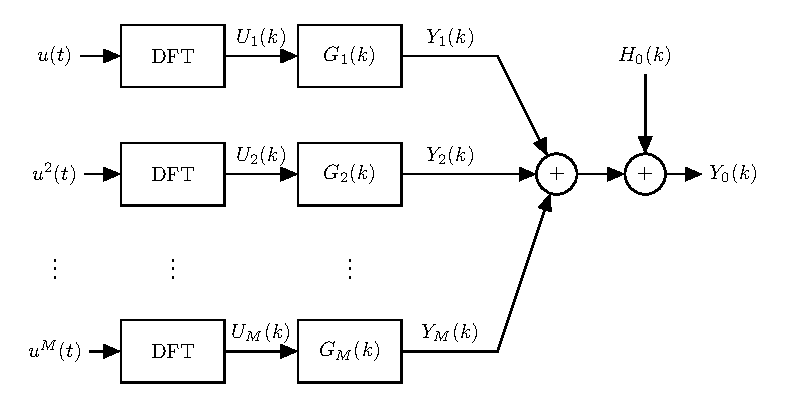
\includegraphics[width=0.9\textwidth]{Chapter7_NOFRFs/NOFRF_blockstructure}
\caption{Equivalent block structure of the NOFRF model}
\label{fig:NOFRF_ModelStructure_Chap7}
\end{figure}

In this chapter, for estimation, the model will also include additive white Gaussian measurement noise at the output. Thus, the \emph{observed} output spectrum is given by
\begin{equation}
\label{eq:NOFRF_Noisy}
Y(k) = Y_0(k) + E(k),
\end{equation} 
where $E(k)$ is assumed i.i.d. with augmented covariance $\sigma^2 I$.

\subsection{The parallel Hammerstein case}

The NOFRFs are input-dependent in general, since they act on exponents of the input rather than the input directly. There exist some special cases in which the frequency functions become independent of the applied input, notably when the system has a parallel Hammerstein structure with polynomial nonlinearities. This structure is depicted in Figure \ref{fig:PolynomialHamm}, where there are $L$ distinct Hammerstein branches, and each branch has a nonlinearity with maximum degree less than or equal to $M$. 

\begin{figure}[h]
\centering
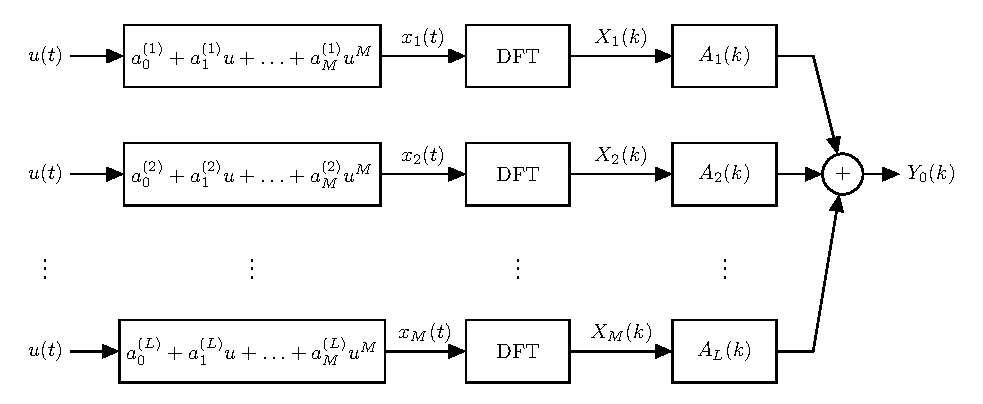
\includegraphics[width=\textwidth]{Chapter7_NOFRFs/ParallelHammStructure}
\caption{Frequency domain block structure of a parallel Hammerstein system with polynomial nonlinearities}
\label{fig:PolynomialHamm}
\end{figure}

To understand why the NOFRFs of such a system are input-independent, the structure can be rearranged by exploiting the linearity of the DFT and the filters, $A_1, A_2, \hdots, A_L$. An alternate parallel Hammerstein block structure is given in Figure \ref{fig:AlternateHamm}, where each exponent of the input is collected in a separate branch, and $H_0(k)$ is a zero frequency contribution produced by the polynomial constants, $a_0^{(i)}, \; \; i = 1,\hdots,L$.  Clearly, this alternate structure matches the NOFRF model structure in Figure \ref{fig:NOFRF_ModelStructure_Chap7}, where the NOFRFs are replaced by 
\begin{equation}
G_m = a_m^{(1)}A_1 + \hdots + a_m^{(L)}A_L \; \; \; m = 1,2,\hdots,M.
\end{equation} 
Thus, for a parallel Hammerstein system, the NOFRFs are linear combinations of the filters from each branch, and since the original filters are all linear and input-independent, the resulting NOFRFs must be also. This is the case which will be considered in the current chapter, where the NOFRFs can be treated as linear filters for identification, and the resulting model will be valid regardless of the system input. 

\begin{figure}[h]
\centering
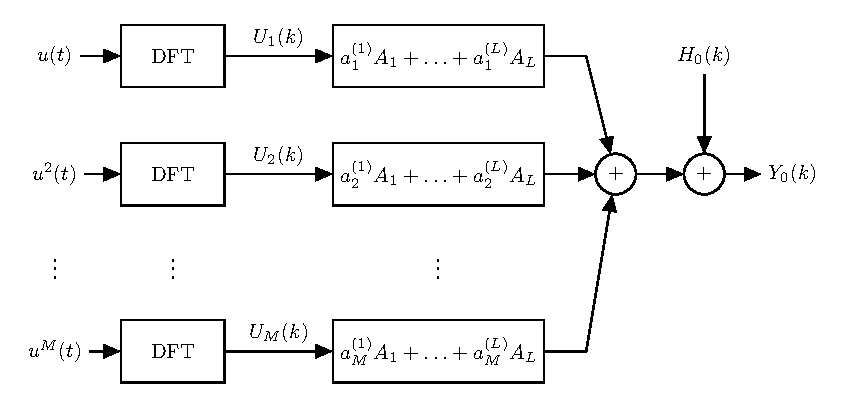
\includegraphics[width=\textwidth]{Chapter7_NOFRFs/AlternateParallelHammStructure}
\caption{Alternate block structure for the parallel Hammerstein system}
\label{fig:AlternateHamm}
\end{figure}

%--------------------------------------------------------------------------------------------------------------------------------------------------------------------------------------------------------

\section{Identification using multi-level excitation}
\label{sec:NOFRFS_multilevel}

The introduction of the NOFRF model in \cite{Lang2005} was accompanied by a data-driven identification scheme. The proposed method requires the system to be excited multiple times by scaled versions of a prototype input signal. Labelling the unscaled prototype input as $u^*(t)$, the set of applied input signals is given by,
$$\beta_i u^*(t), \ \ \ \ i = 1, \hdots, q, \; \; \beta_i \in \mathbb{R}^+,$$
where $q \geq M$ is the total number of excitation levels used. The excitations will produce $q$ corresponding output frequency responses which are denoted as $Y^{(q)}(k)$.

Given the model structure in (\ref{eq:NOFRF_Noisy}), a regression model can be formed at each frequency bin, $k$, using the $q$ excitations applied to the system. These models have the form,
\begin{equation}
\mathbf{Y}(k) = \mathbf{U^*}(k) \mathbf{G}(k) + E,
\label{eq:NOFRF_regressionmodel}
\end{equation}
where
\begin{align}
\mathbf{Y}(k) = \begin{bmatrix} Y^{(1)}(k) \\ \vdots \\ Y^{(q)}(k)\end{bmatrix}, \; \; \mathbf{U^*}(k) = \begin{bmatrix} \beta_1 U^*_1(k) & \hdots & \beta_1^M U^*_M(k) \\ \vdots &\ddots & \vdots \\ \beta_q U^*_1(k) & \hdots & \beta_q^M U^*_M(k) \end{bmatrix}, \; \; \mathbf{G}(k) = \begin{bmatrix} G_1(k) \\ \vdots \\ G_M(k)\end{bmatrix},
\end{align} 
and $U^*_1,\hdots,U^*_M$ are the nonlinear spectral quantities in (\ref{eq:NOFRF_TransientFree_Chap7}) corresponding to $u^*(t)$. 

Least squares estimates for the NOFRFs can be obtained analytically from (\ref{eq:NOFRF_regressionmodel}) at any given frequency. If the error vector $E$ is circular complex distributed, the solution is given as
\begin{equation}
\hat{\mathbf{G}}(k) = \bigg( \big[ \mathbf{U^*}(k) \big]^H \big[ \mathbf{U^*}(k) \big] \bigg)^{-1} \big[ \mathbf{U^*}(k) \big]^H \mathbf{Y}(k) \; \; \; \forall k \in \mathcal{K}
\end{equation}
where $\mathcal{K}$ is the set of excited frequency bins in the input, $U^*_1(k)$. For any other distribution of $E$, (\ref{eq:NOFRF_regressionmodel}) must be separated into its real and imaginary parts, with each part solved separately in the traditional least squares sense (see \cite{Lang2005}).  

This multi-level excitation method for NOFRF estimation has several disadvantages:
\begin{itemize}
\item Data collection may take a long time to perform, requiring at least $M$ experiments which must reach steady-state before measuring.
\item The method cannot be used in cases where the input is not precisely controlled.
\item Least squares solutions are sensitive to measurement noise.
\item The quantity and value of scaling parameters, $\beta_i$, are arbitrary choices which are made by the user.
\end{itemize}
These shortcomings highlight the need for a more sophisticated algorithm, capable of accurate parameter estimation in a generic and noisy experimental setting. In the case of parallel Hammerstein systems, such an algorithm will be developed in the sequel.

%--------------------------------------------------------------------------------------------------------------------------------------------------------------------------------------------------------

\section{Gaussian process regression for NOFRFs}
\label{sec:NOFRFs_GPR}

Taking inspiration from the linear case in \cite{Lataire2016}, an estimation method can be developed from the Bayesian perspective. The NOFRF quantities will be modeled as real/complex parameter vectors with Gaussian prior covariances and estimated using empirical Bayes techniques. To achieve this, some assumptions and notation must first be clarified. 

\begin{assum}[Parallel Hammerstein structure]
\label{ass:HammersteinPolynomial}
The system of interest can be represented by a parallel Hammerstein structure with polynomial nonlinearities of known maximum degree, $M$. Hence, there exist nonzero NOFRFs up to the $M$\textsuperscript{th} nonlinear order.
\end{assum}

\begin{rem}
In the case where $M$ is unknown, or the nonlinearities are not polynomial in nature, there are many established order selection methods, e.g. cross-validation, which can be applied to select an appropriate $M$. 
\end{rem}

\begin{notation}
Let $\mathbf{k}$ be the vector of DFT bins, $k$, for which the input spectrum $U(k)$ is nonzero due to excitation. The corresponding parameter vector to be estimated for the $m$\textsuperscript{th} order NOFRF will be denoted $G_m(\mathbf{k})$.
\end{notation}

\begin{rem}
\label{rem:NOFRFrealpart}
In the parallel Hammerstein case, all NOFRFs $G_m(k)$ will only be strictly real for $k=0$, since they behave like linear filters. The same is true for the measured output, $Y(k)$. 
\end{rem}

\begin{assum}[Independent Gaussian NOFRFs]
\label{ass:GaussianNOFRFs}
Assume that each NOFRF parameter vector is a RCG process with zero mean, i.e.
\begin{equation}
\begin{split}
\label{eq:NOFRF_GaussianDist}
G_m(\mathbf{k}) &\sim \mathcal{RCN}(0,c_{G,m} \Sigma_m), \ \ \ m=1,\hdots,M, \\
H_0(0) &\sim \mathcal{RCN}(0,c_{G,0}),
\end{split}
\end{equation}
where $c_{G,m} \in \mathbb{R}^+$ are normalization hyperparameters, and $\Sigma_m$ are augmented covariances constructed from the covariance and relation matrices, $R_m$, $Q_m$, $K_m$ and $C_m$ as in (\ref{eq:RCNdistribution_defn}). Furthermore, assume that all NOFRFs are independent of each other.
\end{assum}

Recalling that parallel Hammerstein NOFRFs can be interpreted as linear filters, we are free to use the same covariance structures for $\Sigma_m$ as were used in \cite{Lataire2016} for FRF estimation. In this chapter we consider the frequency domain equivalent of the DC structure in (\ref{eq:DCstructure}), whose form is provided in \cite{Lataire2016}\footnote{The transformation of time domain prior covariance structures to the frequency domain will be discussed in more detail in Chapter \ref{chap:8}}. More specifically, the covariance and relation matrices for the RCG process $G_m(\mathbf{k})$ can be constructed using,
\begin{align}
\mathbf{E} \{ G_m(k_x) \overline{G_m(k_y)} \} &= \frac{1}{\lambda_m + j(k_x - k_y)} \Bigg( \frac{1}{\rho_m+\lambda_m/2+jk_x} + \frac{1}{\rho_m + \lambda_m/2 - jk_y} \Bigg), \label{eq:NOFRF_DC1}\\
\mathbf{E} \{ G_m(k_x) G_m(k_y) \} &= \frac{1}{\lambda_m + j(k_x + k_y)} \Bigg( \frac{1}{\rho_m+\lambda_m/2+jk_x} + \frac{1}{\rho_m + \lambda_m/2 + jk_y} \Bigg), \label{eq:NOFRF_DC2}
\end{align}
where $\lambda_m$ and $\rho_m$ are the DC hyperparameters which require tuning.

\subsection{Deriving the MAP estimate}

\begin{assum}[No strictly real components]
For simplicity and mathematical convenience, the remainder of this chapter will assume that the zero frequency bin is not excited, i.e. $0 \notin \mathbf{k}$. As noted in Remark \ref{rem:NOFRFrealpart}, this implies that there are no strictly real components in the vectors $G_m(\mathbf{k})$ and $Y(\mathbf{k})$. Consequently, the real/complex normal framework in Section \ref{sec:RCN} will reduce to the complex normal framework, i.e. $X^{\mathbb{R}}$ is an empty vector in (\ref{eq:augvector_defn}). 
\label{ass:NOFRFs_NoReals}
\end{assum}

In order to derive the Bayesian posterior estimates for each NOFRF, an expression for the output spectrum distribution is first developed.
\begin{thm}%[Output Spectrum Distribution]
For the NOFRF model defined in (\ref{eq:NOFRF_TransientFree_Chap7}) and (\ref{eq:NOFRF_Noisy}) with $G_m$ given by (\ref{eq:NOFRF_GaussianDist}), the vectorized output spectrum, $Y(\mathbf{k})$, is distributed as,
\begin{equation}
\begin{split}
\label{eq:OutputSpectrumThm}
Y(\mathbf{k}) &\sim \mathcal{RCN}(0,\Sigma_Y), \\
\text{where } \Sigma_Y &= \sum_{m=1}^{M} \Sigma_{Y,m} + \sigma^2 I, \\
\text{and } \Sigma_{Y,m} &= c_{G,m} (\widetilde{U_m(\mathbf{k})} \widetilde{U_m(\mathbf{k})}^H)  \circ \Sigma_m.
\end{split}
\end{equation}
\end{thm}
\begin{proof*}
Noting that (\ref{eq:NOFRF_TransientFree_Chap7}) implies $Y_m(\mathbf{k}) = G_m(\mathbf{k}) \circ U_m(\mathbf{k})$, the result follows directly from Assumption \ref{ass:GaussianNOFRFs} and Properties \ref{prop:IndSum} and \ref{prop:HadProd} \hfill $\qed$
\end{proof*}

The NOFRF parameter vectors are now jointly distributed with $Y(\mathbf{k})$, and the Bayesian framework allows computation of maximum a posteriori (MAP) estimates for each $G_m$.%, as shown in the following theorem.

\begin{thm}
\label{thm:NOFRF_MAP_G}
Under Assumptions \ref{ass:HammersteinPolynomial} and \ref{ass:GaussianNOFRFs}, the MAP estimate of $G_m(\mathbf{k})$ is given by,
\begin{equation}
\label{eq:NOFRF_MAP_G}
\hat{\widetilde{G_m(\mathbf{k})}} = c_{G,m} \Sigma_m \diag \big( \widetilde{U_m(\bold{k})}^H \big) \Sigma_Y^{-1} \widetilde{Y(\bold{k})}, 
\end{equation}
where $\diag(X)$ denotes a diagonal matrix with diagonal $X$.
\end{thm}
\begin{proof*}
Acknowledging the independence of each NOFRF, the $m$\textsuperscript{th} order NOFRF and output spectrum are jointly distributed as,
\begin{equation}
\begin{bmatrix}
G_m(\mathbf{k}) \\ Y(\mathbf{k})
\end{bmatrix} \sim \mathcal{RCN} \Bigg( 
\begin{bmatrix}
0 \\ 0
\end{bmatrix},
\begin{bmatrix}
\Sigma_m & \Sigma_{G_m Y}\\ 
\Sigma_{Y G_m} & \Sigma_Y
\end{bmatrix} \Bigg),
\end{equation}
where the joint covariance is computed as,
\begin{align}
\Sigma_{G_m Y} &= \mathbf{E}\Big\{ \widetilde{G_m(\mathbf{k})} \widetilde{Y(\mathbf{k})}^H \Big\} \nonumber \\
&= \mathbf{E}\Big\{ \widetilde{G_m(\mathbf{k})} \Big[ \widetilde{G_m(\mathbf{k})}^H \circ \widetilde{U_m(\mathbf{k})}^H \Big] \Big\} \nonumber \\
&= \mathbf{E}\Big\{ \widetilde{G_m(\mathbf{k})} \widetilde{G_m(\mathbf{k})}^H \Big\} \cdot \diag \big( \widetilde{U_m(\mathbf{k})}^H \big)  \nonumber \\
&= c_{G,m} \Sigma_m \diag \big( \widetilde{U_m(\mathbf{k})}^H \big), \label{Sigma_GmY}
\end{align}
using (\ref{eq:NOFRF_TransientFree_Chap7}), (\ref{eq:NOFRF_Noisy}) and Assumption \ref{ass:GaussianNOFRFs}. Now the MAP estimate will be the mean of the conditional distribution, $G_m(\mathbf{k})|Y(\mathbf{k})$, which is given by Property \ref{prop:CondDist} as
\begin{equation}
\label{eq:NOFRF_MAP}
\mathbf{E} \Big\{ \widetilde{G_m(\mathbf{k})}|\widetilde{Y(\mathbf{k})} \Big\} = \Sigma_{G_m Y} \Sigma_Y^{-1} \widetilde{Y(\mathbf{k})}.
\end{equation}
Combining (\ref{eq:NOFRF_MAP}) with (\ref{Sigma_GmY}) yields the result in (\ref{eq:NOFRF_MAP_G}). \hfill $\qed$
\end{proof*}

\subsection{Hyperparameter tuning}

As in all Bayesian estimation methods discussed in this thesis, the hyperparameters describing the covariance of each NOFRF must be empirically tuned prior to estimation. For an $M$\textsuperscript{th} order model, the DC hyperparameter vector will be
\begin{align*}
\eta &= [\sigma^2 \ \eta_1 \ \hdots \ \eta_M], \\
\text{where }\eta_m &= [c_{G,m} \ \lambda_m \ \rho_m].
\end{align*}
In this chapter, as in \cite{Lataire2016}, the tuning process is achieved by maximizing the marginal log likelihood of the hyperparameters with respect to the observed output, i.e.
\begin{equation}
\label{eq:NOFRF_HyperparamTuning}
\hat{\eta} = \text{arg } \underset{\eta}{\text{min }} \widetilde{Y(\mathbf{k})}^H \Sigma_Y^{-1}(\eta) \widetilde{Y(\mathbf{k})} + \log \det \Sigma_Y(\eta).
\end{equation} 

%--------------------------------------------------------------------------------------------------------------------------------------------------------------------------------------------------------

\section{GPR estimation in the presence of transients}
\label{sec:NOFRF_TransientEstimation}

Unlike the traditional multi-level excitation method, the Gaussian process regression approach can be modified to remove the effect of transient functions in estimation, allowing identification of NOFRFs in the case of non-periodic or non-steady-state measurement data.

It was shown in \cite{Lataire2016} that in the linear case, transient functions result from the difference $f(t) = u(t)-u(t+N)$ for $-\infty<t<0$. Considering now the NOFRF case and observing Figure \ref{fig:NOFRF_ModelStructure_Chap7}, it is clear that for a non-periodic $u(t)$, $u^m(t)$ will also be non-periodic, and there will be a transient function at each nonlinear order. We can use this information to update the model equation in (\ref{eq:NOFRF_TransientFree_Chap7}) as follows:
\begin{equation}
Y_0(k) = H_0(k) + \sum_{m=1}^{M} G_m(k) U_m(k) + T_m(k),
\end{equation}
where $T_m(k)$ is the $m$\textsuperscript{th} order transient function in the frequency domain. 

In general, it is not obvious what kind of Gaussian prior is appropriate for a transient function. However, for the case of a zero mean white noise input it has been shown in \cite{Lataire2016} that for linear systems, the prior covariance of the transient function is approximately proportional to the system covariance. This result also extends to the NOFRF case for parallel Hammerstein systems, as can be confirmed by observing Figure \ref{fig:NOFRF_ModelStructure_Chap7}. Whenever $u(t)$ is white noise we will have, in each branch, a transient produced by non-periodic white noise $u^m(t)$ passing through a linear filter $G_m$. Consequently, the following Gaussian assumptions will be placed on the transient vectors.
\begin{assum}
Given a white noise input, the distribution of the $m$\textsuperscript{th} order transient vector is given by,
\begin{equation}
T_m(\mathbf{k}) \sim \mathcal{RCN}(0,c_{T,m} \Sigma_m),
\end{equation}
where $c_{T,m} \in \mathbb{R}^+$ is a normalization hyperparameter, and $\Sigma_m$ is the augmented covariance of NOFRF vector $G_m(\mathbf{k})$.
\end{assum}
\begin{assum}
The transient vectors at each nonlinear order, $m$, are independent of each other and all NOFRF vectors.
\end{assum}

The distribution of the output spectrum can now be updated accordingly, giving
\begin{equation}
\begin{split}
\label{eq:OutputSpectrumWithTransients}
\Sigma_Y &= \sum_{m=1}^{M} \Sigma_{Y,m} + \sigma^2 I, \\
\Sigma_{Y,m} &= c_{G,m} (\widetilde{U_m(\mathbf{k})} \widetilde{U_m(\mathbf{k})}^H)  \circ \Sigma_m + c_{T,m} \Sigma_m.
\end{split}
\end{equation}

Hyperparameter tuning can still be performed using (\ref{eq:NOFRF_HyperparamTuning}), with additional hyperparameters in the optimization, i.e. $$\eta_m = [c_{G,m} \ c_{T,m} \ \lambda_m \ \rho_m].$$

Finally, the MAP estimates for each $G_m(\mathbf{k})$ will remain as in Theorem \ref{thm:NOFRF_MAP_G}, using the updated definition of $\Sigma_Y$ in (\ref{eq:OutputSpectrumWithTransients}). Furthermore, MAP estimates of the transient functions can also be obtained using the same logic, yielding
\begin{equation}
\hat{\widetilde{T_m(\mathbf{k})}} = c_{T,m} \Sigma_m  \Sigma_Y^{-1} \widetilde{Y(\mathbf{k})}.
\end{equation} 

%--------------------------------------------------------------------------------------------------------------------------------------------------------------------------------------------------------

\section{GPR estimation using multiple input realizations}
\label{sec:NOFRF_MultipleRealizations}

If a set of NOFRFs are estimated using only \emph{one} input realization, as in (\ref{eq:NOFRF_MAP_G}), then the estimation problem is inevitably underdetermined. This is because for every measurement, $Y(k)$, in the output spectrum, we must estimate the value of multiple NOFRFs at that same frequency. The GPR framework is flexible enough to handle this case and produce reasonable estimates, however the accuracy of the estimates will improve if the ratio of measurement data to model parameters is increased.

In frequency domain estimation problems, the typical method for increasing the amount of measurement data is to perform multiple experiments, each with a different input realization. Indeed, this concept was required for the multi-level excitation method in Section \ref{sec:NOFRFS_multilevel}, where each input realization was a scaled version of some prototype signal. In this section we will present an extension to the GPR method developed in Section \ref{sec:NOFRFs_GPR}, which considers multiple input/output realizations in the estimation.

\begin{assum}
There are $q$ separate realizations of transient-free input/output measurement data available, with a shared vector, $\mathbf{k}$, of excited DFT frequencies.
\label{ass:NOFRFs_multiplerealz}
\end{assum}

\begin{notation}
The $i$\textsuperscript{th} realization has input and output spectrum measurements given by $Y^{(i)}(\mathbf{k})$ and $U^{(i)}(\mathbf{k})$ respectively. The associated vectors containing all realizations are denoted by
\begin{equation}
\mathbf{Y}(\mathbf{k}) = \begin{bmatrix} Y^{(1)}(\mathbf{k}) \\ \vdots \\ Y^{(q)}(\mathbf{k})\end{bmatrix} \textrm{ and } \mathbf{U}_m(\mathbf{k}) = \begin{bmatrix} U_m^{(1)}(\mathbf{k}) \\ \vdots \\ U_m^{(q)}(\mathbf{k}) \end{bmatrix} \textrm{ for } m = 1,\hdots,M.
\end{equation}
\label{not:NOFRFs_multiplerealz}
\end{notation}

Noting Assumptions \ref{ass:NOFRFs_NoReals} and \ref{ass:NOFRFs_multiplerealz} as well as Notation \ref{not:NOFRFs_multiplerealz}, and using the NOFRF model (\ref{eq:NOFRF_TransientFree_Chap7}), the model equation for multiple realizations can be written as
\begin{equation}
\mathbf{Y}(\mathbf{k}) = \sum_{m=1}^M \Big[ \underbrace{G_m(\mathbf{k}) \; \; \hdots \; \; G_m(\mathbf{k})}_{q \textrm{ copies}} \Big]^T \circ \mathbf{U}_m(\mathbf{k}).
\label{eq:NOFRFs_RegressionMultipleRealz}
\end{equation}
Now with the new model structure (\ref{eq:NOFRFs_RegressionMultipleRealz}) and recalling Assumption \ref{ass:GaussianNOFRFs}, the GPR method in Section \ref{sec:NOFRFs_GPR} can be applied with the following modifications.

The distribution of $\mathbf{Y}(\mathbf{k})$ is given by
\begin{equation}
\begin{split}
\label{eq:MultipleOutputSpectrumThm}
\mathbf{Y}(\mathbf{k}) &\sim \mathcal{RCN}(0,\mathbf{\Sigma}_Y), \\
\text{where } \mathbf{\Sigma}_Y &= \sum_{m=1}^{M} \mathbf{\Sigma}_{Y,m} + \sigma^2 I, \\
\mathbf{\Sigma}_{Y,m} &= c_{G,m} (\widetilde{\mathbf{U}_m(\mathbf{k})} \widetilde{\mathbf{U}_m(\mathbf{k})}^H)  \circ \mathbf{\Sigma}_m.
\end{split}
\end{equation}
Recall the covariance and relation matrices, $K_m$ and $C_m$, of $\Sigma_m$, which can be constructed using the transformed DC structure (\ref{eq:NOFRF_DC1}) and (\ref{eq:NOFRF_DC2}). The matrix $\mathbf{\Sigma}_m$ is constructed using its own covariance and relation matrices, $\mathbf{K}_m$ and $\mathbf{C}_m$, whose form is easily found as
\begin{equation}
\mathbf{K}_m = \underbrace{\begin{bmatrix} K_m & \hdots & K_m \\ \vdots & \ddots & \vdots \\ K_m & \hdots & K_m \end{bmatrix}}_{q \times q \textrm{ copies}}, \; \; \mathbf{C}_m = \underbrace{\begin{bmatrix} C_m & \hdots & C_m \\ \vdots & \ddots & \vdots \\ C_m & \hdots & C_m \end{bmatrix}}_{q \times q \textrm{ copies}}.
\end{equation}

The MAP estimate of $G_m(\mathbf{k})$ now becomes
\begin{equation}
\label{eq:NOFRF_MAP_G_MultRealz}
\hat{\widetilde{G_m(\mathbf{k})}} = c_{G,m} \underbrace{\begin{bmatrix} K_m & \hdots & K_m & C_m & \hdots & C_m \\ C_m^H & \hdots & C_m^H & \overline{K_m} & \hdots & \overline{K_m} \end{bmatrix}}_{q \textrm{ copies of each}} \diag \big( \widetilde{\mathbf{U}_m(\mathbf{k})}^H \big) \mathbf{\Sigma}_Y^{-1} \widetilde{\mathbf{Y}(\mathbf{k})}, 
\end{equation}
and hyperparameter tuning is achieved using
\begin{equation}
\label{eq:NOFRF_HyperparamTuning_MultRealz}
\hat{\eta} = \text{arg } \underset{\eta}{\text{min }} \widetilde{\mathbf{Y}(\mathbf{k})}^H \mathbf{\Sigma}_Y^{-1}(\eta) \widetilde{\mathbf{Y}(\mathbf{k})} + \log \det \mathbf{\Sigma}_Y(\eta).
\end{equation} 

%--------------------------------------------------------------------------------------------------------------------------------------------------------------------------------------------------------

\section{Simulation examples}

Numerical simulations are performed in this section to compare the performance of the proposed GPR method, which we will refer to as \emph{regularized}, against the \emph{traditional} method of multi-level excitation. Using a Monte Carlo approach, the methods are compared for varying noise levels and number of NOFRFs. 

The GPR method is also applied to simulated experimental data which is not in steady-state. In these examples, output transient functions are estimated via the proposed Bayesian framework and compared against the true observed transient.

\subsection{Simulation settings}

All simulations use the parallel Hammerstein structure shown in Figure \ref{fig:ParallelHammNumEx}, which is intentionally constructed such that each parallel branch contains only one exponent of the input in its nonlinear block. With such a structure, the NOFRFs are directly equal to the linear filter in their corresponding branch. Note that each branch can be switched in and out of the system depending on the experiment settings.

\begin{figure}[h]
\centering
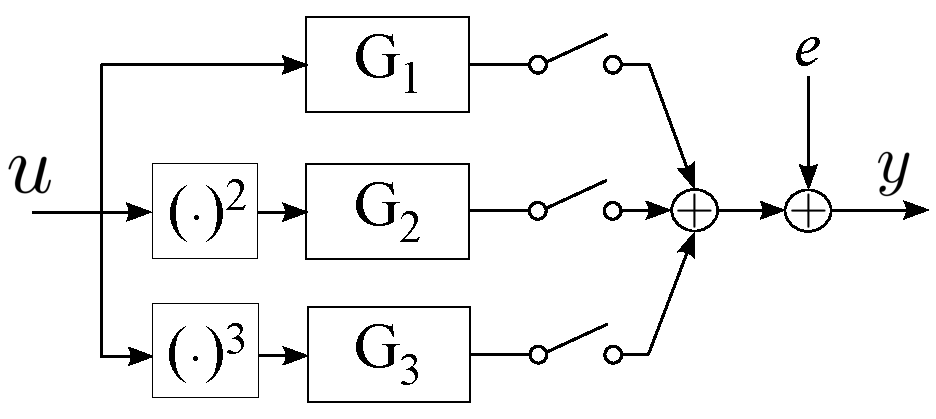
\includegraphics[width=0.5\textwidth]{Chapter7_NOFRFs/ParallelHammNumEx.pdf}
\caption{Parallel Hammerstein structure used for numerical examples}
\label{fig:ParallelHammNumEx}
\end{figure}

In the simulation, the linear filters (and therefore the NOFRFs), $G_1$, $G_2$ and $G_3$, are constructed as Chebyshev filters with resonant modes at normalized frequencies 0.072, 0.111 and 0.091 respectively. The inputs in any given experiment are random-phase multisines which are periodic in $N=128$ samples and have no zero frequency component. The band of excitation, $\mathbf{k}$, for the multisines is constructed so as to avoid aliasing in the output spectrum. The output error, $e$, is a Gaussian white noise vector added in each experiment to provide the required signal-to-noise ratio (SNR).

\subsection{Comparison of traditional and GPR methods}

Four 1000-run Monte Carlo studies are performed on the traditional and regularized estimation methods to determine their relative accuracy.  The studies are:
\begin{enumerate}
\item $M=2$ ($G_1$ and $G_2$ branches) with SNR = 40dB. 1 input/output realization for the \emph{regularized} method. 2 input scalings for the \emph{traditional} method. 
\item $M=2$ ($G_1$ and $G_2$ branches) with SNR = 20dB. 1 input/output realization for the \emph{regularized} method. 2 input scalings for the \emph{traditional} method. 
\item $M=3$ (all branches) with SNR = 40dB. 1 input/output realization for the \emph{regularized} method. 3 input scalings for the \emph{traditional} method. 
\item $M=3$ (all branches) with SNR = 40dB. 10 input/output realizations for the \emph{regularized} method. 10 input scalings for the \emph{traditional} method. 
\end{enumerate}

Note that for studies 1, 2 and 3, the traditional multi-level excitation method uses its minimum requirement of $M$ differently scaled inputs, and hence $M$ experiments. In contrast, the regularized method is disadvantaged in these studies by using only one input and experiment, such that data collection is faster by a factor of $M$. Furthermore, the estimation is performed on a dataset which is smaller by a factor of $M$ for the GPR method. The final study (4) compares the two methods for an equal amount of measurement data, using the results in Section \ref{sec:NOFRF_MultipleRealizations} for the regularized method. For a fair comparison of the two methods, all studies use measurement data taken from the steady-state portion of the experiment, i.e. there are no transient components in the output response. 

To visualize performance in each Monte Carlo study, Figures \ref{fig:NOFRFs_2ndOrder_SNR100}, \ref{fig:NOFRFs_2ndOrder_SNR10}, \ref{fig:NOFRFs_3rdOrder_SNR100} and \ref{fig:NOFRFs_3rdOrder_SNR100_10times} plot the true NOFRF magnitudes as well as the central 95\% intervals (shaded) from each estimation method. For studies 1, 2 and 3, the regularized method produces tighter intervals which are more centered around the true NOFRF, despite having a shorter experiment time and using significantly less data in the estimation. The contrast in performance is even clearer in the results for study 4, where the regularized method is allowed to use an equal amount of measurement data. All of the Monte Carlo results show a clear accuracy benefit for the proposed method when output measurement noise is present in the system, which can be attributed to the ability of GPR methods to significantly reduce estimation covariance at the price of a small bias \citep{Pillonetto2014}. The bias here is small but evident, particularly at the resonance peaks of each NOFRF.

\begin{figure}[!hp]
\centering
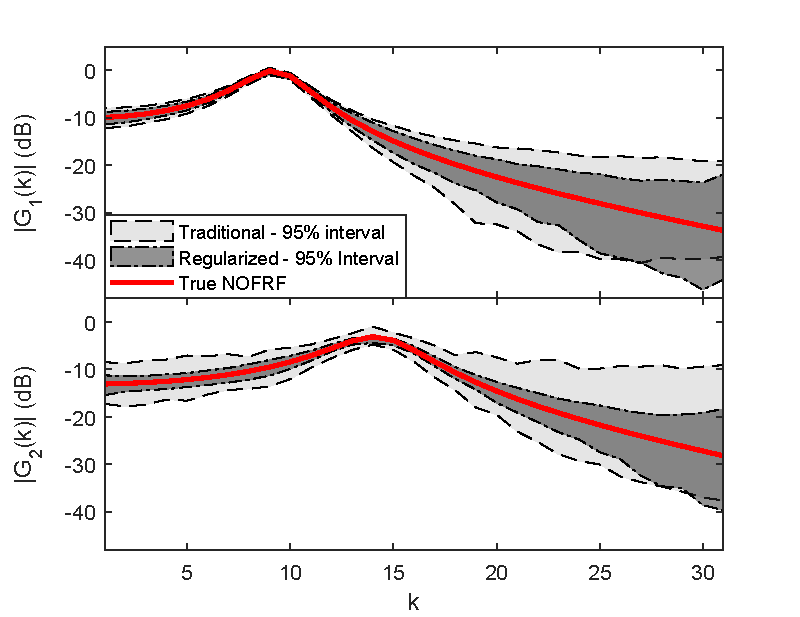
\includegraphics[width=0.8\textwidth]{Chapter7_NOFRFs/Hamm2ndOrder_SNR100_N128_DiscreteTime.pdf}
\caption{Magnitude intervals for study 1, $M=2$ and SNR=40dB}
\label{fig:NOFRFs_2ndOrder_SNR100}
\end{figure}

\begin{figure}[!hp]
\centering
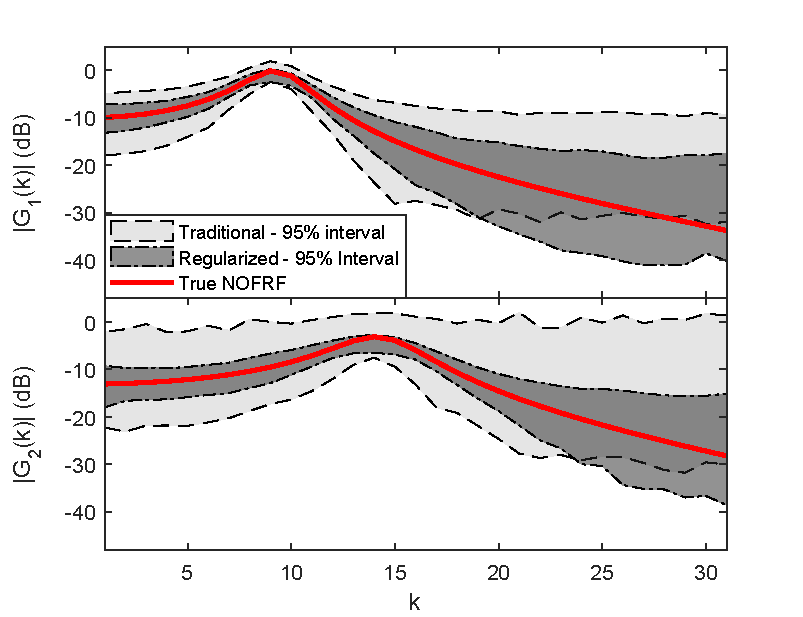
\includegraphics[width=0.8\textwidth]{Chapter7_NOFRFs/Hamm2ndOrder_SNR10_N128_DiscreteTime.pdf}
\caption{Magnitude intervals for study 2, $M=2$ and SNR=20dB}
\label{fig:NOFRFs_2ndOrder_SNR10}
\end{figure}

\begin{figure}[!hp]
\centering
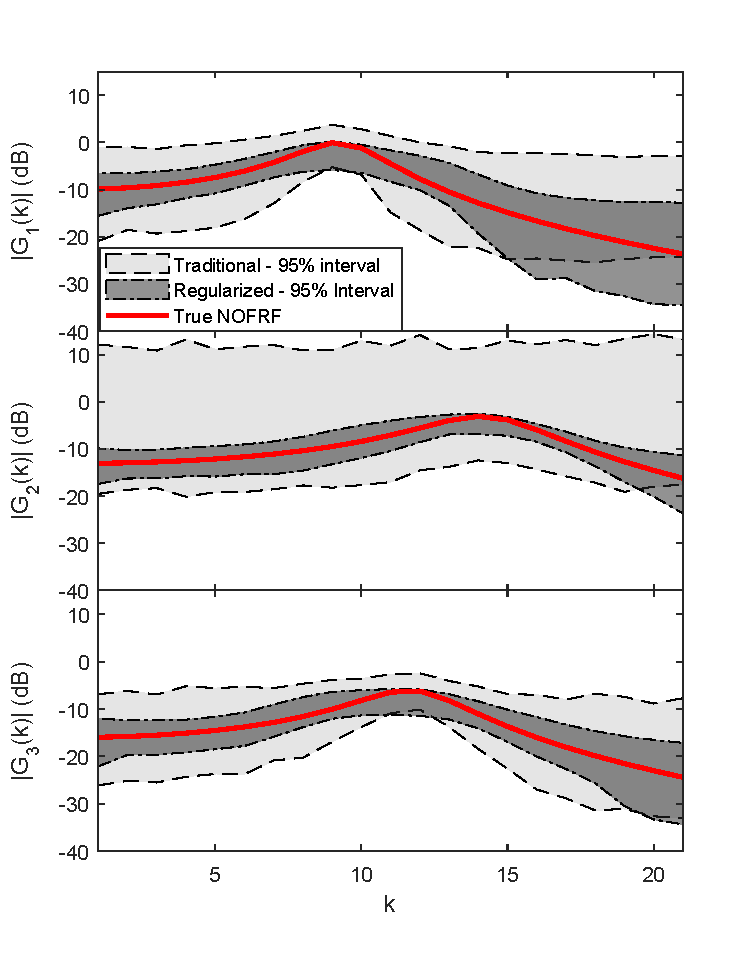
\includegraphics[width=0.6\textwidth]{Chapter7_NOFRFs/Hamm3rdOrder_SNR100_N128_DiscreteTime.pdf}
\caption{Magnitude intervals for study 3, $M=3$ and SNR=40dB}
\label{fig:NOFRFs_3rdOrder_SNR100}
\end{figure}

\begin{figure}[!hp]
\centering
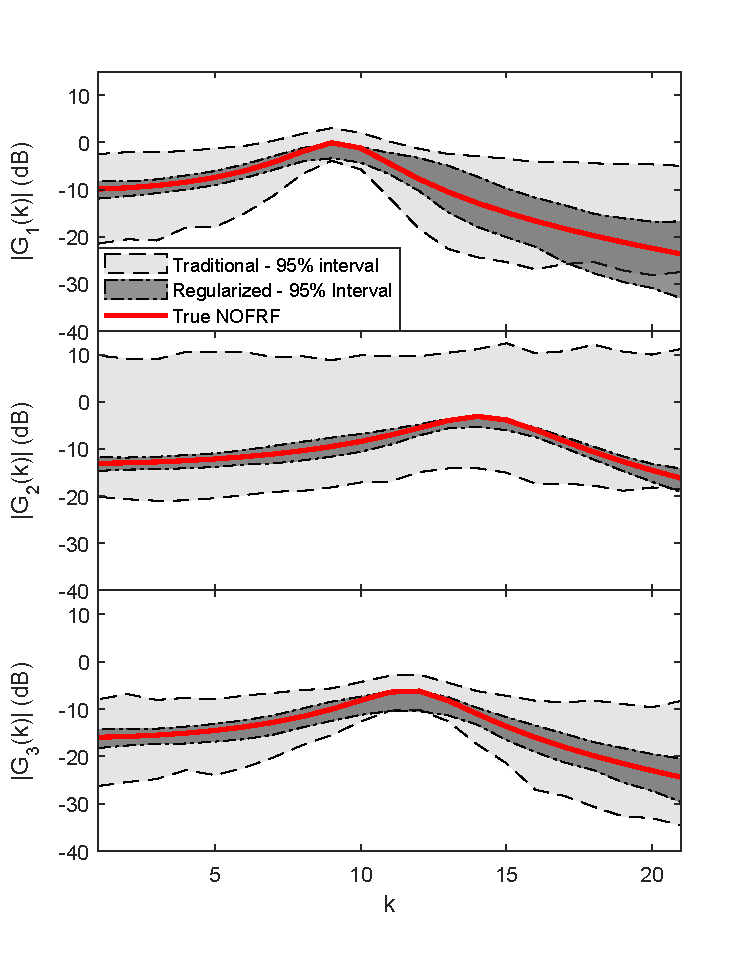
\includegraphics[width=0.6\textwidth]{Chapter7_NOFRFs/Hamm3rdOrder_SNR100_10timesN128_DiscreteTime.pdf}
\caption{Magnitude intervals for study 4, $M=3$ and SNR=40dB (equal data)}
\label{fig:NOFRFs_3rdOrder_SNR100_10times}
\end{figure}

\subsection{Transient estimation test}

While the traditional multi-level excitation method cannot estimate or remove the effect of transients, it was shown in Section \ref{sec:NOFRF_TransientEstimation} that the proposed approach can be modified to consider transient functions in the Gaussian process regression. This allows us to simultaneously estimate the NOFRFs and their corresponding transients, thereby increasing the accuracy of estimation for non-periodic or non steady-state data. 

To demonstrate this capability, the modified method in Section \ref{sec:NOFRF_TransientEstimation} was applied to the simulated system of Figure \ref{fig:ParallelHammNumEx}, using the $G_1$ and $G_2$ branches and no output noise. The input multisine was applied for a single period and preceded by zero initial conditions, producing a transient in the output response. Using this input/output data, the total transient could be estimated by summing the transient estimates from each nonlinear order, i.e.
\begin{equation}
T(k) = \sum_{m=1}^{M} T_m(k).
\end{equation}
The true and estimated transients are plotted in Figure \ref{fig:NOFRFTransientEstimates} for three input realizations, showing reasonable estimation performance which significantly reduces the effect of the transients on NOFRF estimation accuracy. 

\begin{figure}[h]
\centering
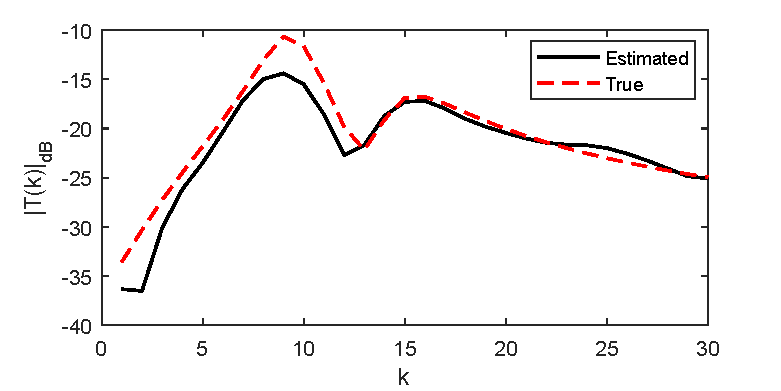
\includegraphics[width=0.7\textwidth]{Chapter7_NOFRFs/NOFRF_Transient1.pdf}
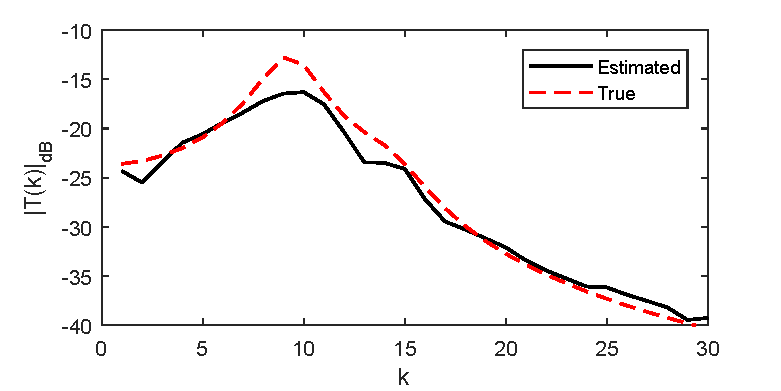
\includegraphics[width=0.7\textwidth]{Chapter7_NOFRFs/NOFRF_Transient4.pdf}
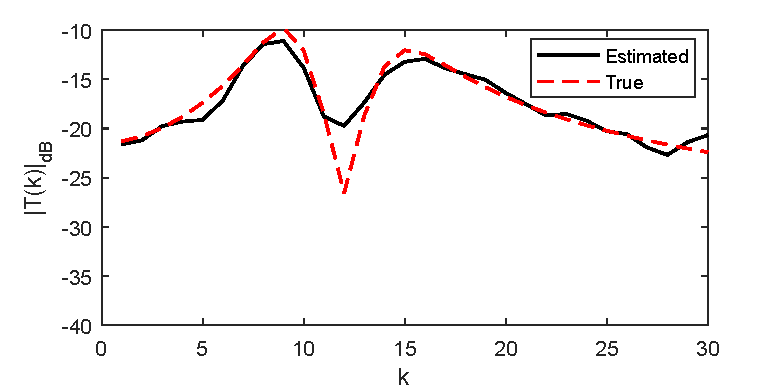
\includegraphics[width=0.7\textwidth]{Chapter7_NOFRFs/NOFRF_Transient5.pdf}
\caption{True and estimated transient functions for three input realizations of the test system ($M=2$)}
\label{fig:NOFRFTransientEstimates}
\end{figure}

\section{Conclusion}

This chapter adapts the Bayesian techniques from linear identification theory to the problem of estimating parallel Hammerstein systems in the frequency domain. First, the NOFRF model structure was shown to be an intuitive and useful tool in estimating such systems, since the frequency function at each nonlinear order will be input-independent and pseudo-linear for this case. In developing a GPR method, the Gaussian prior covariances for each frequency function could then be chosen and tuned according to results obtained for linear FRF estimation in~\cite{Lataire2016}. The proposed method was extended to consider concurrent transient estimation in the case of non-steady-state data. When compared to the traditional NOFRF estimation method of multi-level excitation, the proposed method has fewer experimental constraints and can achieve higher accuracy using less data when output noise is present. 

In order to estimate frequency domain models for a broader class of nonlinear systems, the NOFRF method proposed in this chapter would not be sufficient. This is because the NOFRFs are input-dependent in general, and thus we cannot always impose prior covariance structures borrowed from the linear theory. An alternate option is to move to the multidimensional GFRF model structure, and design an analogous method to the regularized Volterra kernel estimation outlined in Chapter \ref{sec:RegVolterraTD}. Such an approach will be considered in Chapter \ref{chap:8}.